%% This is file `elsarticle-template-1-num.tex',
%%
%% Copyright 2009 Elsevier Ltd
%%
%% This file is part of the 'Elsarticle Bundle'.
%% ---------------------------------------------
%%
%% It may be distributed under the conditions of the LaTeX Project Public
%% License, either version 1.2 of this license or (at your option) any
%% later version.  The latest version of this license is in
%%    http://www.latex-project.org/lppl.txt
%% and version 1.2 or later is part of all distributions of LaTeX
%% version 1999/12/01 or later.
%%
%% The list of all files belonging to the 'Elsarticle Bundle' is
%% given in the file `manifest.txt'.
%%
%% Template article for Elsevier's document class `elsarticle'
%% with numbered style bibliographic references
%%
%% $Id: elsarticle-template-1-num.tex 149 2009-10-08 05:01:15Z rishi $
%% $URL: http://lenova.river-valley.com/svn/elsbst/trunk/elsarticle-template-1-num.tex $
%%
\documentclass[preprint,12pt]{elsarticle}

%% Use the option review to obtain double line spacing
%% \documentclass[preprint,review,12pt]{elsarticle}

%% Use the options 1p,twocolumn; 3p; 3p,twocolumn; 5p; or 5p,twocolumn
%% for a journal layout:
%% \documentclass[final,1p,times]{elsarticle}
%% \documentclass[final,1p,times,twocolumn]{elsarticle}
%% \documentclass[final,3p,times]{elsarticle}
%% \documentclass[final,3p,times,twocolumn]{elsarticle}
%% \documentclass[final,5p,times]{elsarticle}
%% \documentclass[final,5p,times,twocolumn]{elsarticle}

%% if you use PostScript figures in your article
%% use the graphics package for simple commands
%% \usepackage{graphics}
%% or use the graphicx package for more complicated commands
%% \usepackage{graphicx}
%% or use the epsfig package if you prefer to use the old commands
%% \usepackage{epsfig}

%% The amssymb package provides various useful mathematical symbols
\usepackage{amssymb}
%% The amsthm package provides extended theorem environments
%% \usepackage{amsthm}

%% The lineno packages adds line numbers. Start line numbering with
%% \begin{linenumbers}, end it with \end{linenumbers}. Or switch it on
%% for the whole article with \linenumbers after \end{frontmatter}.
\usepackage{lineno}

%% natbib.sty is loaded by default. However, natbib options can be
%% provided with \biboptions{...} command. Following options are
%% valid:

%%   round  -  round parentheses are used (default)
%%   square -  square brackets are used   [option]
%%   curly  -  curly braces are used      {option}
%%   angle  -  angle brackets are used    <option>
%%   semicolon  -  multiple citations separated by semi-colon
%%   colon  - same as semicolon, an earlier confusion
%%   comma  -  separated by comma
%%   numbers-  selects numerical citations
%%   super  -  numerical citations as superscripts
%%   sort   -  sorts multiple citations according to order in ref. list
%%   sort&compress   -  like sort, but also compresses numerical citations
%%   compress - compresses without sorting
%%
%% \biboptions{comma,round}

% \biboptions{}
\usepackage[utf8]{inputenc}
\usepackage[T1]{fontenc}
%\usepackage[english]{babel}


 % Formátování čísel
\usepackage[autolanguage]{numprint}
\usepackage[detect-none]{siunitx}
\sisetup{range-phrase = \text{ -- }}
\npdefunit{nm}{nm}{0.00000035145980351}

 % Znak pro teplotu \celsius
\usepackage{gensymb}

 % Proklíkávací odkazy
\usepackage{hyperref}
\usepackage[capitalise]{cleveref}





\newcommand{\luag}{LuAG:Pr$^{3+}$@SiO$_{2}$-PPIX}
\newcommand{\azid}{NaN$_{3}$}
\newcommand{\znoo}{ZnO:Ga@SiO$_{2}$-PPIX}
\newcommand{\singlet}{$^{1}$O$_{2}$}



\journal{English Course}

\begin{document}

\begin{frontmatter}

%% Title, authors and addresses

%% use the tnoteref command within \title for footnotes;
%% use the tnotetext command for the associated footnote;
%% use the fnref command within \author or \address for footnotes;
%% use the fntext command for the associated footnote;
%% use the corref command within \author for corresponding author footnotes;
%% use the cortext command for the associated footnote;
%% use the ead command for the email address,
%% and the form \ead[url] for the home page:
%%
%% \title{Title\tnoteref{label1}}
%% \tnotetext[label1]{}
%% \author{Name\corref{cor1}\fnref{label2}}
%% \ead{email address}
%% \ead[url]{home page}
%% \fntext[label2]{}
%% \cortext[cor1]{}
%% \address{Address\fnref{label3}}
%% \fntext[label3]{}

\title{Investigation of nanomaterials for singlet oxygen production}

%% use optional labels to link authors explicitly to addresses:
%% \author[label1,label2]{<author name>}
%% \address[label1]{<address>}
%% \address[label2]{<address>}

\author{Iveta Terezie Pelikánová$^{a}$, Lenka Procházková$^{a}$, Kseniya Popovich$^{a}$, Kateřina Tomanová$^{a}$, Václav Čuba$^{a}$, Eva Mihóková$^{b}$, Ivo Jakubec$^{c}$, Roman Dědic$^{d}$ and Martin Nikl$^{b}$}

\address{
    $^{a}$Department of Nuclear Chemistry, Faculty of Nuclear Sciences and Physical Engineering, Czech Technical University in Prague, Břehová 7, Prague 115 19, Czech Republic\\ 
    $^{b}$Department of Optical Materials, Institute of Physics of the Czech Academy of Sciences, Cukrovarnická 10, Prague 162 53, Czech Republic\\
    $^{c}$Institute of Inorganic Chemistry of the Czech Academy of Sciences, Husinec-Řež 1001, Řež 250 68, Czech Republic\\
    $^{d}$Charles University, Faculty of Math and Physics, Ke Karlovu 3, 121 16, Prague, Czech Republic}


\begin{abstract}

%% Text of abstract

Luminescent nanocomposite material, ZnO:Ga@SiO$_{2}$-PPIX, for singlet oxygen production and detection is investigated in this work. Photo-induced method and two step biofunctionalization were used for preparation of the material. Nanoparticles were coated with silica and conjugated with PPIX. XRDP, electron microscopy, RL and PL emission spectra and PL decay were carried out to characterize the materials. Fluorescent probe APF and singlet oxygen quencher {\azid} were used for monitoring the singlet oxygen production. XRDP diffraction patterns prove that biofunctionalization do not change the patterns. And luminescent measurement of APF denotes effective singlet oxygen production during X-ray irradiation of the nanocomposite material.

\end{abstract}

\begin{keyword}
    singlet oxygen \sep nanoparticles \sep luminescence \sep photodynamic therapy \sep zinc oxide
    
%% keywords here, in the form: keyword \sep keyword

%% MSC codes here, in the form: \MSC code \sep code
%% or \MSC[2008] code \sep code (2000 is the default)

\end{keyword}


\end{frontmatter}


%%
%% Start line numbering here if you want
%%
\linenumbers

%% main text

\section{Introduction}
\label{s:introduction}

Nanobiotechnology is an emerging branch of~science that deals with the applications of~nanotechnology in the life sciences \cite{jain10}. Nanomaterials are smaller than the human cells and approximately similar in size to biological macromolecules. Nanoparticles attached to~liposomes, polymers, folic acids, antibodies or peptides improve specific passive or~active drug targeting and efficiency of~medical treatments \cite{lammers08}.   
 
Photodynamic Therapy (PDT) is medical treatment technique based on  photosensitized generation of~singlet oxygen. This technique is used to treat various types of~cancer, e.g. skin, lung, esophagus or stomach cancer, and it is an alternative method to chemotherapy and radiotherapy \cite{rollakanti15,takahashi09}. The biggest limitation for PDT is the use of~visible light in therapeutic window of~\SIrange{600}{900}{nm} to irradiate photosensitizers. These wavelengths penetrate the epidermis but cannot reach deeply located organs or tissues. That is why extensive research of~PDT induced by X-rays (PDTX) is ongoing. Addition of~nanoscintillator enables the use of~X-rays instead of~visible light. Nanoscintillators absorb X-rays and convert them to the visible light in absorption range of~photosensitizer \cite{jary13,chen15}. These changes enhance depth penetration and increase the number of~treatable cancer types. \\

In this work I use zinc oxide doped with gallium (ZnO:Ga) as a nanoscintillator. The surface of nanoparticles is modified by silica coating and protoporphyrin IX (PPIX) is used as a photosensitizer. 


\section{Materials and methods}
\label{s:materials}

    \subsection{Nanoparticle synthesis}
    
        The synthesis of ZnO:Ga was based on previous works \cite{Prochazkova2015,Vanecek2017}. 
        For stock solution of gallium (III) ions \numprint[g]{0.0327} of gallium (III) oxide was dissolved in \numprint[ml]{1} of nitric acid and the solution was topped up to \numprint[ml]{10} by water. 
        \numprint[g]{4.07} of zinc oxide (ZnO) was dissolved in \numprint[ml]{3,9} of formic acid, \numprint[ml]{1} of stock solution and \numprint[ml]{200} of hydrogen peroxide was added and the solution was filled up to \numprint[ml]{2000} by water. Aqueous solution was irradiated by low-pressure mercury lamps for \numprint[min]{100}. 
        Prepared zinc peroxide was separated by filtration, washed by water and EtOH and dried at \numprint[\celsius]{40} in air. The product was recrystallised for \numprint[min]{60} at \numprint[\celsius]{200} and calcined for \numprint[min]{120} at \numprint[\celsius]{1000}. Crystalline ZnO was annealing in reduction atmosphere of~H$_{2}$/Ar mixture (1:20) for \numprint[min]{60} at about \numprint[\celsius]{800}.\\
     
        Surface modification of nanoparticles was based on sol-gel process published in Chemistry of Materials journal \cite{Liu1998} and modified according to Ing.~Vojtěch Vaněček master thesis \cite{Vanecek2017}. Porphyrin nanoconjugates were prepared according to work of Nowostawska et al. \cite{nowostawska11}.

    \subsection{Luminescence and photoluminescence of ZnO:Ga and ZnO:Ga@SiO$_{2}$-PPIX} \label{sec:character_zno}
    
    Radioluminescence spectra were measured with \mbox{X-ray} source on FZU, \numprint[kV]{40} and \numprint[mA]{15}. Approximately \numprint[mg]{15} were dispersed in plastic cuvette with EtOH and the cuvette was placed into the device.
    
    Decay curves and PL emission spectra of ZnO:Ga@SiO$_{2}$-PPIX components were taken to the improved evaluation of results. Steady state deuterium lamp was used to measure PL emission spectra under \numprint[nm]{339} and \numprint[nm]{405} excitation. PL decay curves were measured using nanosecond pulsed LEDs \numprint[nm]{339}, \numprint[nm]{389} and \numprint[nm]{452}. 


    % \subsection{Production of singlet oxygen}  \label{sec:production_singlet}

    % {\singlet} is generated by irradiation of suspension of nanocomposite material in some solvent in the cuvette. Chemical probe APF was used to monitor generation of {\singlet}. The suspension was about \numprint[mg]{15} of powder, about \numprint[ml]{2,5} of solvent and \numprint[$\mu$l]{150} of APF. Monitoring is based on indirect measurement of luminescence of APF. PL emission spectra for \numprint[nm]{470} excitation was measured. Samples were irradiated by X-ray source on Departement of Nuclear Chemistry, \numprint[kV]{40} and \numprint[mA]{15}.
    
    
\section{Results}
\label{s:results}

    The diffraction patterns for ZnO:Ga, ZnO:Ga@SiO$_{2}$ and {\znoo} are shown in \cref{fig:xrdp_znO}. They are all in agreement with that of ZnO:Ga standard (card No. 01-073-1368) from ICDD PDF-2 database. Prepared materials correspond to  hexagonal crystal structure of wurtzite. The absence of additional peaks in diffraction patterns excludes the presence of any other crystalline phase. Narrow diffraction peaks indicates larger crystallites. Electron microscopy confirmed larger crystallites, the size of nanocomposite was at the limit of measurability thus images are a little bit blurred. Scans from scanning electron microscopy are shown in the \cref{fig:sem_znoga,fig:sem_zgs,fig:sem_zgsp}.\\
    
    \begin{figure}
        \centering
        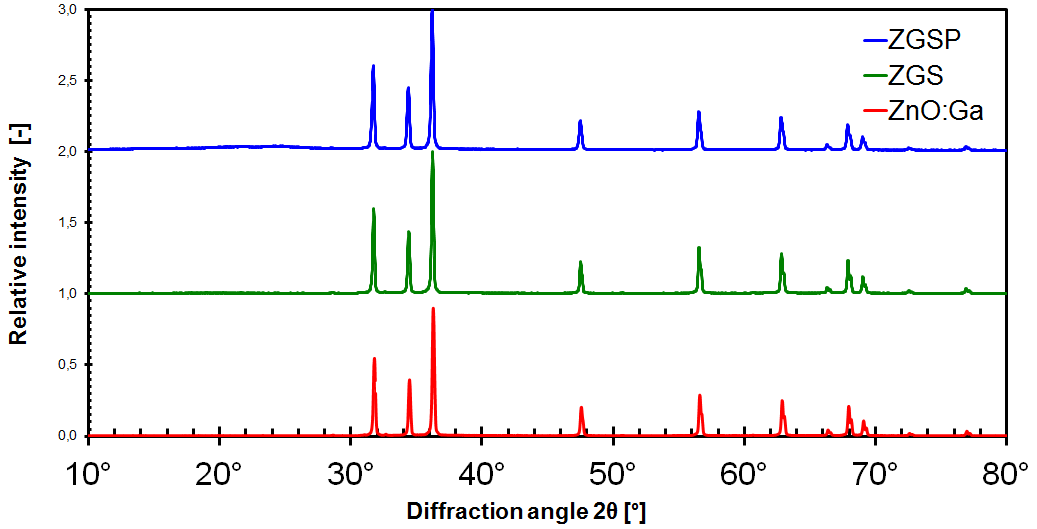
\includegraphics[width=0.8\textwidth]{pictures/xrd_januar_18.PNG}
        \caption{XRDP diffraction patterns of synthesized nanoparticles for ZnO:Ga, ZnO:Ga@SiO$_{2}$ (ZGS) and {\znoo} (ZGSP). Data for ZnO:Ga@SiO$_{2}$ and {\znoo} are vertically shifted for better visualization.}
        \label{fig:xrdp_znO}
    \end{figure}
    
\begin{figure}
    \centering
        \hspace*{\fill}%
    \begin{minipage}{.3\textwidth}
        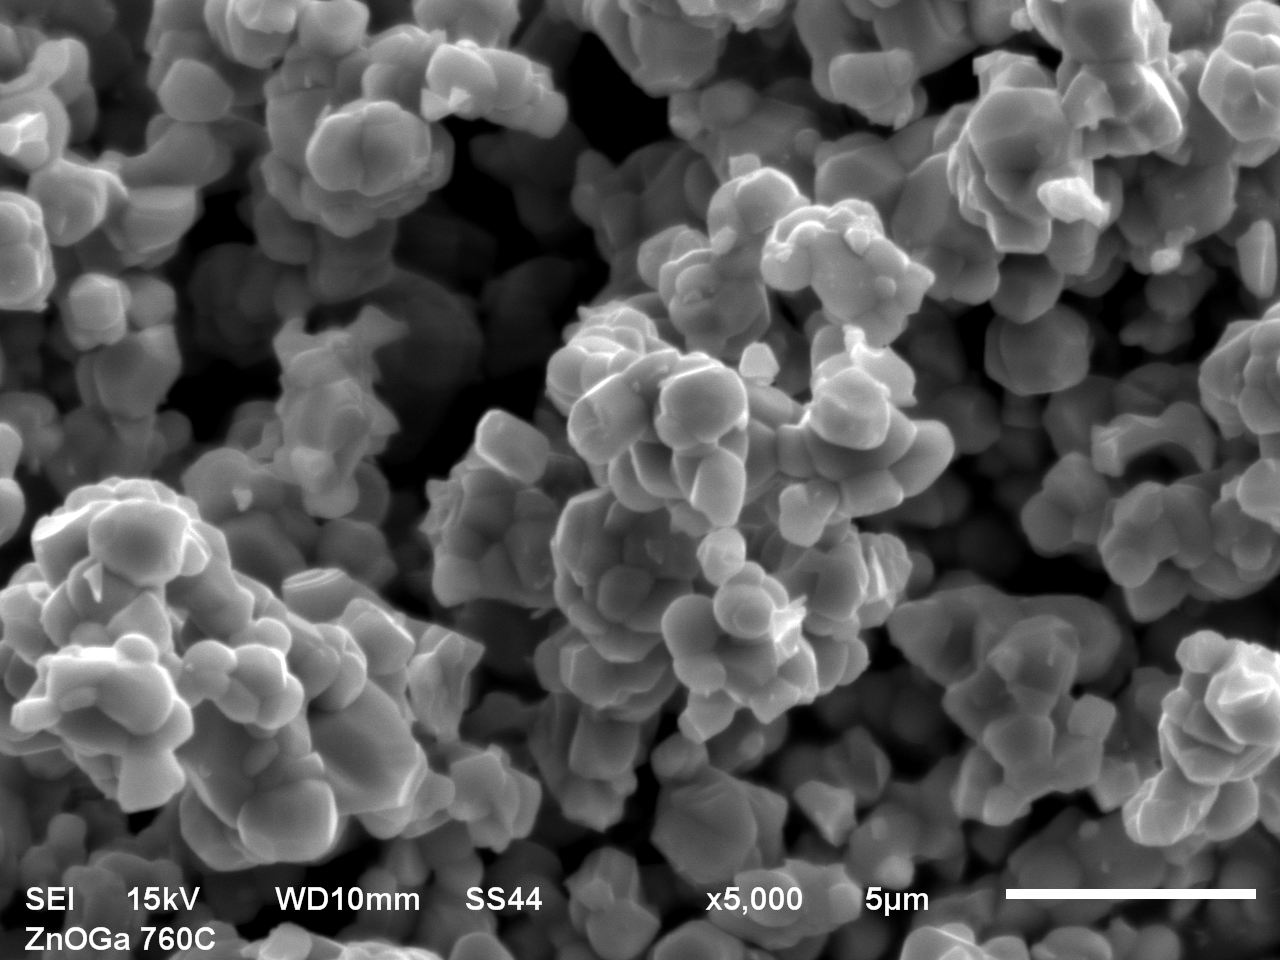
\includegraphics[width=\textwidth]{pictures/sem_ZnOGa_5_mikro.png}
        \caption{SEM scan of ZnO:Ga.}
        \label{fig:sem_znoga}
    \end{minipage}
      \hspace{\fill}%
    \begin{minipage}{.3\textwidth}
        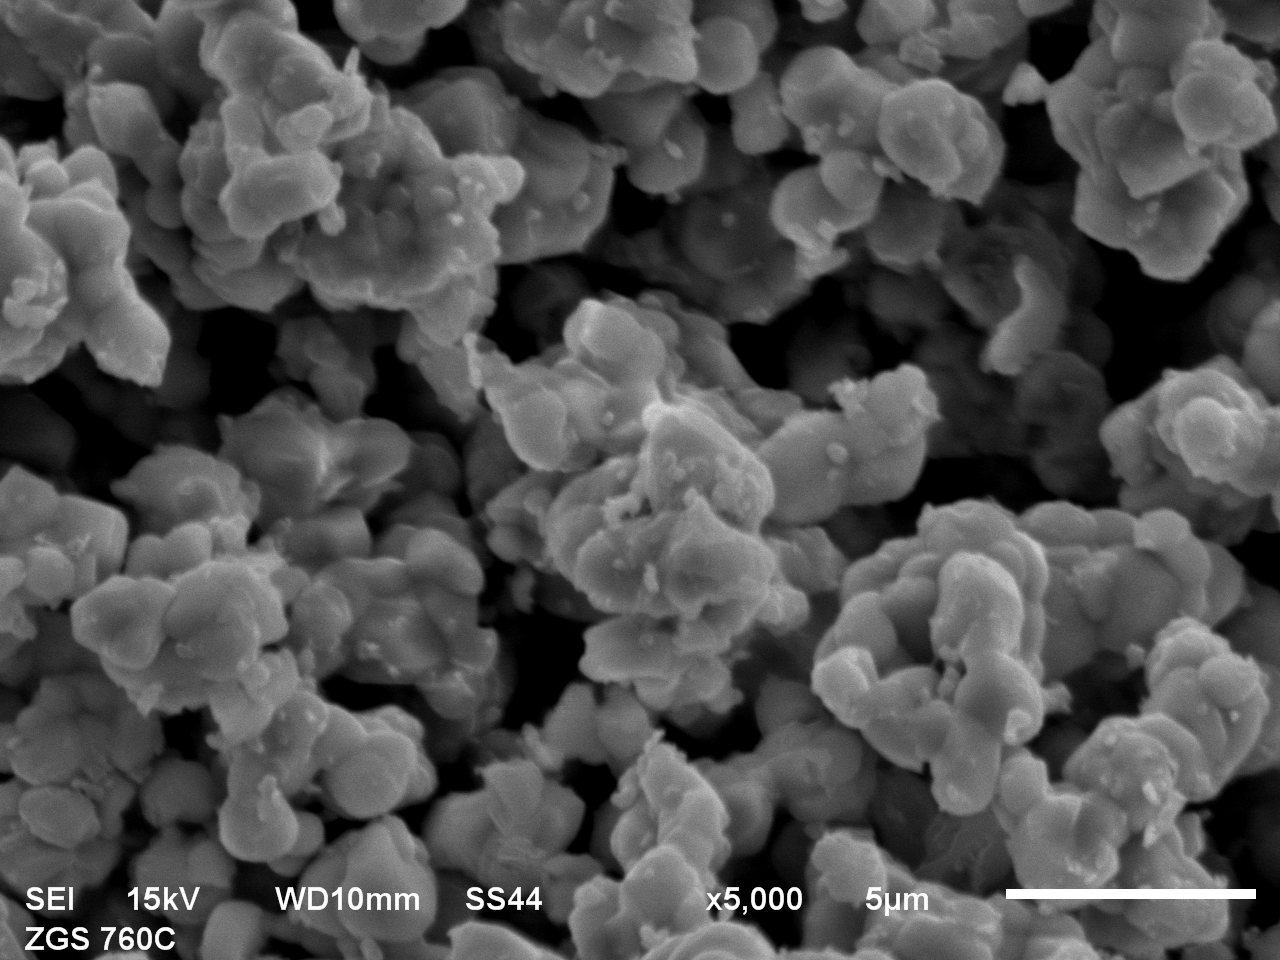
\includegraphics[width=\textwidth]{pictures/sem_ZGS_5_mikro.png}
        \caption{SEM scan of ZnO:Ga@SiO$_{2}$.}
        \label{fig:sem_zgs}
    \end{minipage}
        \hspace*{\fill}%
    \begin{minipage}{.3\textwidth}
        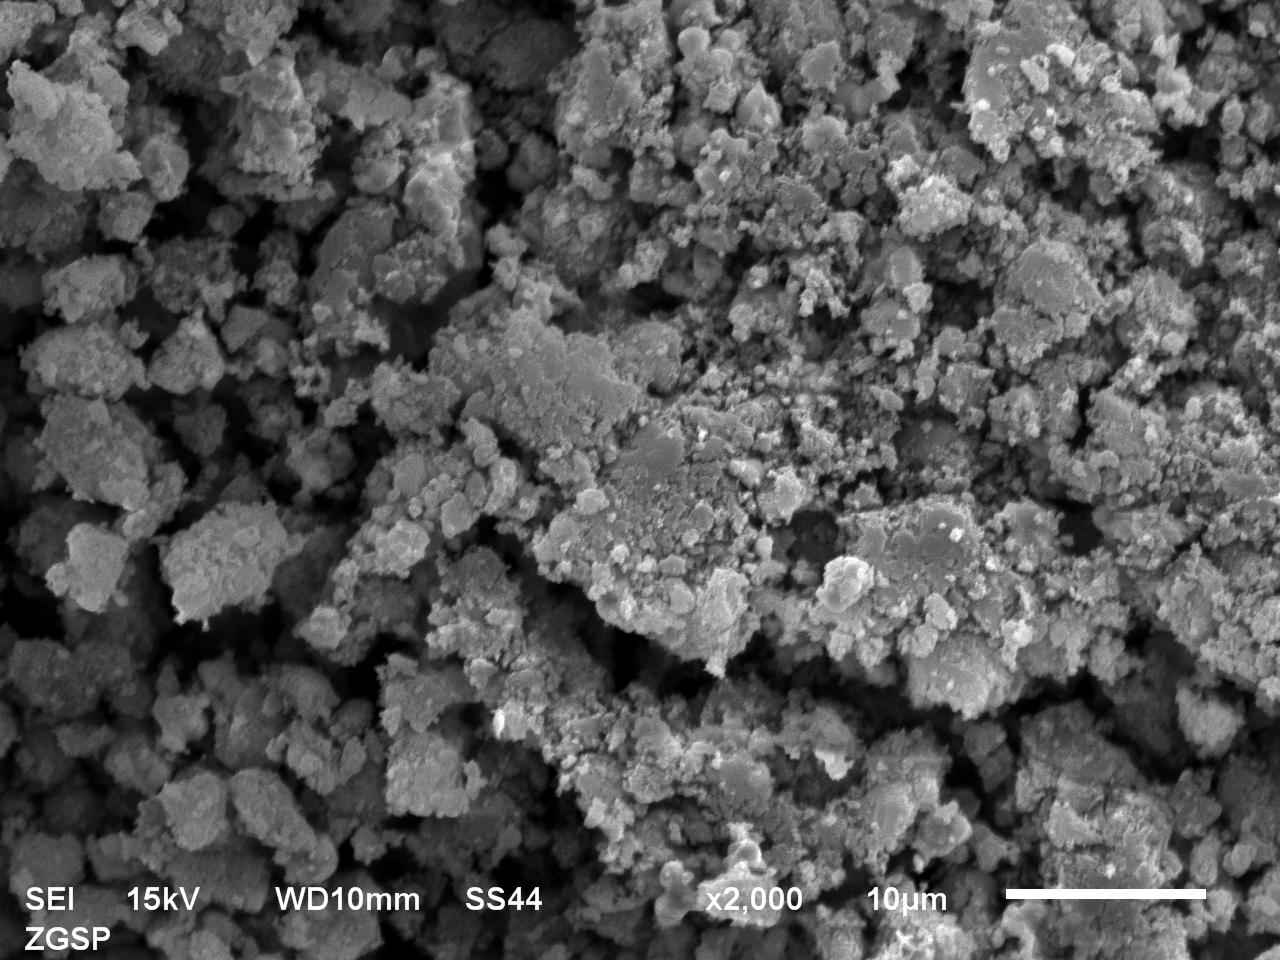
\includegraphics[width=\textwidth]{pictures/sem_ZGSP_10_mikro.png}
        \caption{SEM scan of {\znoo}.}
        \label{fig:sem_zgsp}
    \end{minipage}
        \hspace*{\fill}%
\end{figure}

    The \cref{fig:znoga_januar_rt_pl} shows RL and PL emission spectra of Zno:Ga and {\znoo}. The diffrence in the intensities of luminescence at \numprint[nm]{590} and at \numprint[nm]{650} is observed. This difference is caused by conjugation of PPIX in nanocomposite. It is not clear why PL emission spectrum of {\znoo} do not show any emission peak of ZnO:Ga at \numprint[nm]{390}. Non-radiation energy transfer probably takes place between ZnO:Ga and PPIX since PPIX peaks at \numprint[nm]{590} and \numprint[nm]{650} are observed and emission of ZnO:Ga at \numprint[nm]{390} is not observed.\\
    
    \begin{figure}[h]
        \centering
        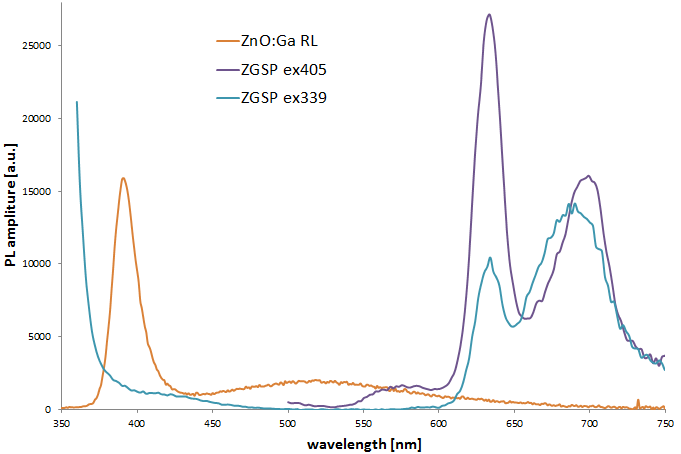
\includegraphics[width=0.6\textwidth]{pictures/znoga_januar_rt_pl.PNG}
        \caption{RL and PL emission spectra of ZnO:Ga and ZnO:Ga@SiO$_{2}$-PPIX (ZGSP) under \numprint[nm]{339} and \numprint[nm]{405} excitation.}
        \label{fig:znoga_januar_rt_pl}
    \end{figure}
    
    
    In addition PL decay curves under \numprint[nm]{339} and \numprint[nm]{389} excitation were measured, they are shown in the \cref{fig:zgs_januar_340ex_390em,fig:zgsp_januar_340ex_390em,fig:zgsp_januar_340ex_630em,fig:zgsp_januar_389ex_630em}. 
    From previous characterization it is obvious that decay time of ZnO:Ga is about \numprint[ns]{0.5} and decay time of PPIX is about \numprint[ns]{3}. 
    The \cref{fig:zgsp_januar_340ex_390em} shows decay time \numprint[ns]{2.4} which belongs to PPIX. 
    In the \cref{fig:zgsp_januar_340ex_630em} and \cref{fig:zgsp_januar_389ex_630em}, decay time of ZnO:Ga@SiO2-PPIX is about \numprint[ns]{12}. 
    This decay times could belong to free PPIX in dilute solution. 
    In comparison with other experiments, it is obvious that the decay times belong to PPIX and not to SiO$_{2}$ shell.
    
    Within the measurements luminescence was really low that could cause unmeasurable conditions or refer to the preparation of the material was not realized correct.\\
    
    \begin{figure}
        \centering
        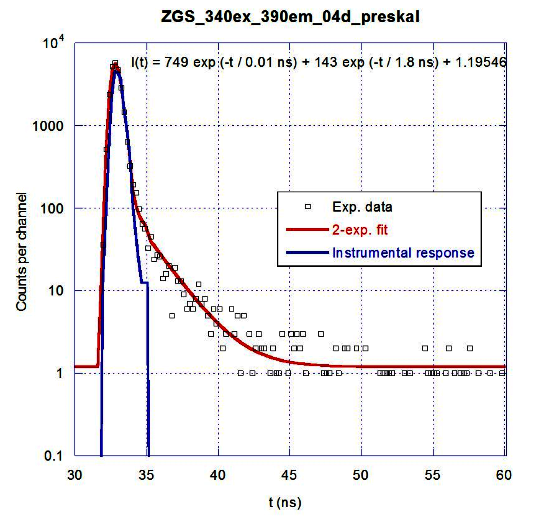
\includegraphics[width=0.6\textwidth]{pictures/zgs_januar_340ex_390em.PNG}
        \caption{PL decay of ZnO:Ga@SiO2 in EtOH under \numprint[nm]{339} excitation, emission \numprint[nm]{390}.}
        \label{fig:zgs_januar_340ex_390em}
    \end{figure}
    
    \begin{figure}
        \centering
        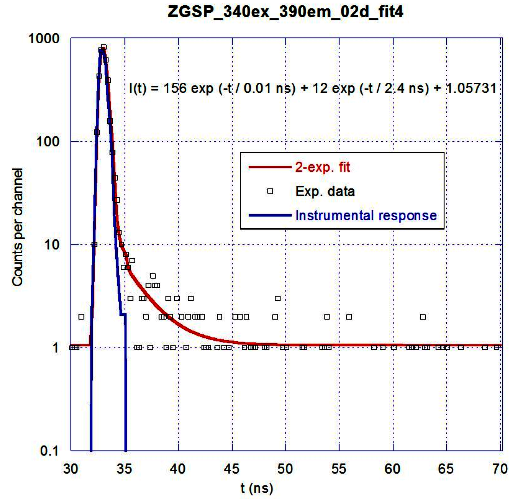
\includegraphics[width=0.6\textwidth]{pictures/zgsp_januar_340ex_390em.PNG}
        \caption{PL decay of {\znoo} in EtOH under \numprint[nm]{339} excitation, emission \numprint[nm]{390}.}
        \label{fig:zgsp_januar_340ex_390em}
    \end{figure}
    
    \begin{figure}
        \centering
        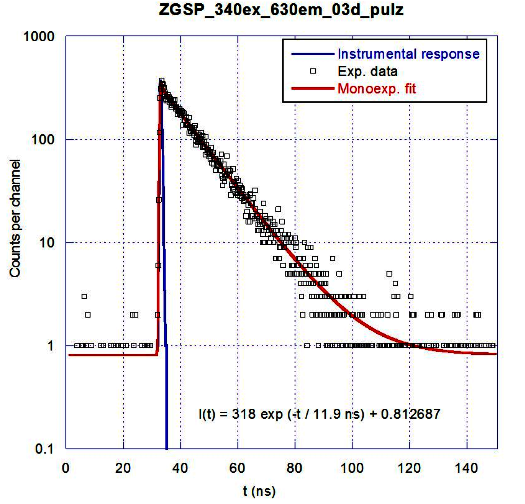
\includegraphics[width=0.6\textwidth]{pictures/zgsp_januar_340ex_630em.PNG}
        \caption{PL decay of {\znoo} in EtOH under \numprint[nm]{339} excitation, emission \numprint[nm]{630}.}
        \label{fig:zgsp_januar_340ex_630em}
    \end{figure}
    
    \begin{figure}
        \centering
        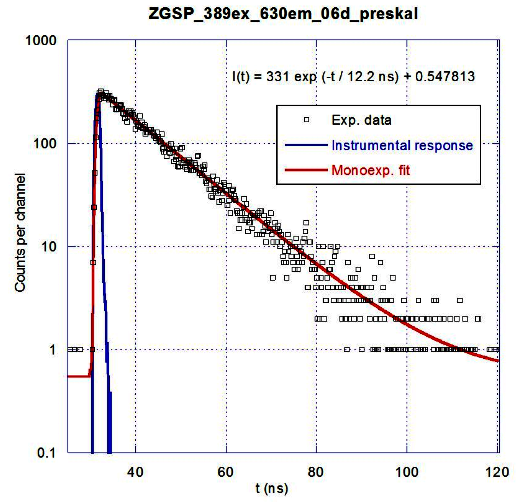
\includegraphics[width=0.6\textwidth]{pictures/zgsp_januar_389ex_630em.PNG}
        \caption{PL decay of {\znoo} in EtOH under \numprint[nm]{389} excitation, emission \numprint[nm]{630}.}
        \label{fig:zgsp_januar_389ex_630em}
    \end{figure}
    
    \subsection{Singlet oxygen production and detection}
    
    {\singlet} generation was investigated after X-ray irradiation of nanocomposite materials in solvent. The APF probe was used to indirect detection of {\singlet}. In short, absorption maximum of APF is at about \numprint[nm]{490} and oxidised form of APF is highly luminescent at \numprint[nm]{515}. Changes in luminescence of APF during irradiation were monitored. APF reacts with {\singlet} and with other ROS, moreover with -OH radicals \cite{bartosz06, setsukinai03}. Sodium azide {\azid} was chosen to distinguish emission which belongs to {\singlet} oxidation and emission which belongs to other ROS oxidisation. {\azid} is specific quencher of {\singlet} \cite{bulin13}. According to research in literature, concentration \numprint[mM]{10} of {\azid} in EtOH was used \cite{price09,bancirova11, huang12, liyi12}.
    
    After biofunctionalization the product consisted of dark coloured and light coloured part. The \cref{fig:xrd_zgsp_dark_fair} shows XRDP diffraction patterns for these two parts and silica coated precursor. It seems that both parts consist of nanoparticles ZnO:Ga. From the \cref{fig:xrdp_znO} it is obvious that diffraction patterns did not change during biofunctionalization. The XRDP pattern for dark coloured part of ZnO:Ga@SiO$_{2}$-PPIX indicates the samples contained a lot of amorphous phase, probably unbounded free PPIX.

        \begin{figure}
        \centering
        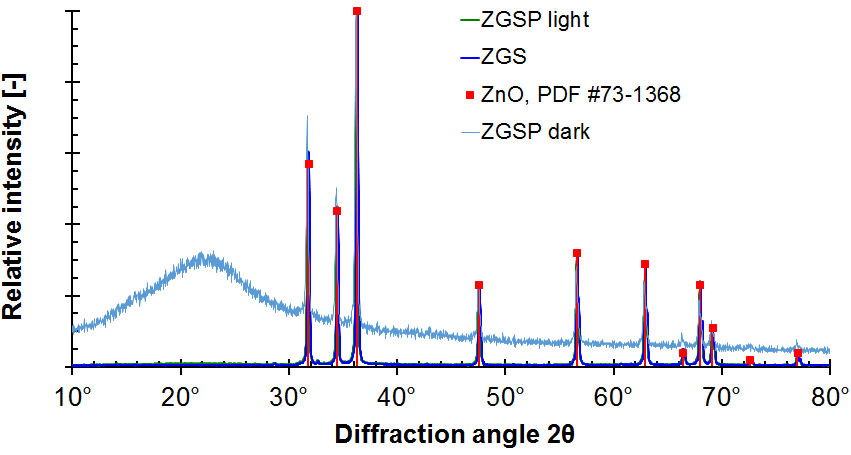
\includegraphics[width=0.6\textwidth]{pictures/xrd_zgsp_dark_fair.PNG}
        \caption{XRDP diffraction patterns for ZnO:Ga@SiO$_{2}$ (ZGS), light coloured part of ZnO:Ga@SiO$_{2}$-PPIX (ZGSP) and dark coloured part of ZnO:Ga@SiO$_{2}$-PPIX (ZGSP dark).}
        \label{fig:xrd_zgsp_dark_fair}
        \end{figure}
    
    The \cref{fig:apf_zgsp_dark_new_holder} shows spectra which belong to the dark coloured part of ZnO:Ga@SiO$_{2}$-PPIX. It is obvious that luminescence intensity decreases in time at peaks \numprint[nm]{590} and \numprint[nm]{650}. No luminescence increase is observed at maximum of APF at \numprint[nm]{520} as shown in the \cref{fig:apf_zgsp_dark_vyrez_new_holder}. The characterization of dark coloured part of ZnO:Ga@SiO$_{2}$-PPIX showed a small amount of ZnO:Ga in the sample, therefore the generation of {\singlet} could have been unmeasurable.

    The \cref{fig:apf_zgsp_fair_new_holder} shows spectra which belong to the light coloured part of ZnO:Ga@SiO$_{2}$-PPIX. Against the \cref{fig:apf_zgsp_dark_new_holder} luminescence intensity increases in time. The \cref{fig:apf_zgsp_fair_vyrez_new_holder} shows changes in APF luminescence in time. Unexpectedly, luminescence at peak \numprint[nm]{640} rises also as shown in the \cref{fig:apf_zgsp_fair_new_holder}. Previous experiments confirm that this peak belongs to PPIX and not to APF. Luminescence at peak \numprint[nm]{640} decreases  in the \cref{fig:apf_zgsp_dark_new_holder} unlike the increase in the \cref{fig:apf_zgsp_fair_new_holder}. The reduction could be caused by sedimentation of the nanocomposite material. We could not explain this luminescence rise in detail. Since measurements with {\azid} were not carried out within these samples we could not prove {\singlet} generation. However, the luminescence increase in the \cref{fig:apf_zgsp_fair_vyrez_new_holder} denotes {\singlet} production in time.

    \begin{figure}
        \centering
        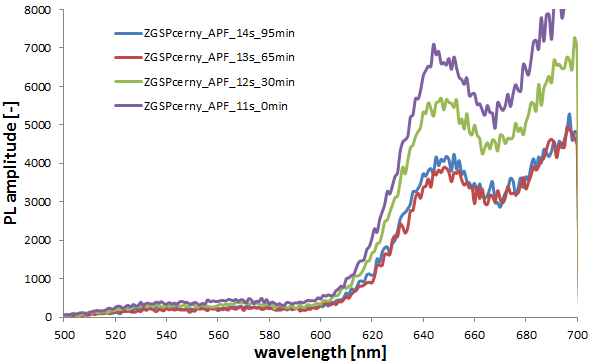
\includegraphics[width=0.6\textwidth]{pictures/apf_zgsp_dark_new_holder.PNG}
        \caption{PL emission spectra of dark coloured part of ZnO:Ga@SiO$_{2}$-PPIX (ZGSP) in EtOH under \numprint[nm]{470} excitation.}
        \label{fig:apf_zgsp_dark_new_holder}
    \end{figure}
    
    \begin{figure}
        \centering
        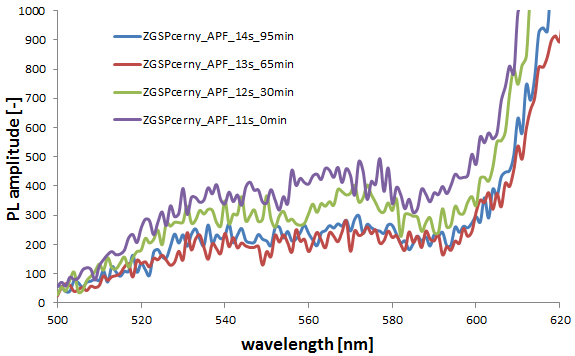
\includegraphics[width=0.6\textwidth]{pictures/apf_zgsp_dark_vyrez_new_holder.PNG}
        \caption{PL emission spectra of dark coloured part of ZnO:Ga@SiO$_{2}$-PPIX in EtOH under \numprint[nm]{470} excitation, monitoring APF.}
        \label{fig:apf_zgsp_dark_vyrez_new_holder}
    \end{figure}
    
    \begin{figure}
        \centering
        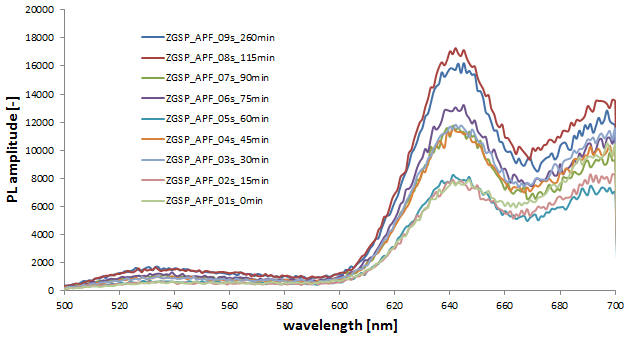
\includegraphics[width=0.6\textwidth]{pictures/apf_zgsp_fair_new_holder.PNG}
        \caption{PL emission spectra of light coloured part of ZnO:Ga@SiO$_{2}$-PPIX (ZGSP) in EtOH under \numprint[nm]{470} excitation.}
        \label{fig:apf_zgsp_fair_new_holder}
    \end{figure}
    
    \begin{figure}
        \centering
        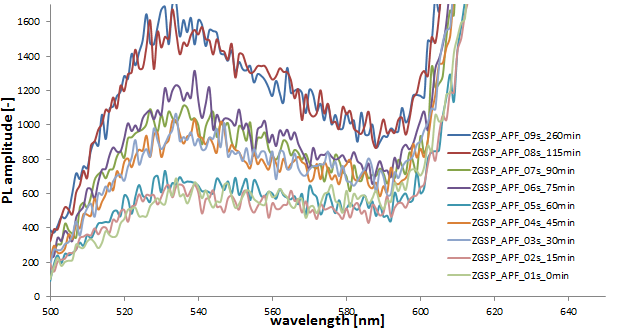
\includegraphics[width=0.6\textwidth]{pictures/apf_zgsp_fair_vyrez_new_holder.PNG}
        \caption{PL emission spectra of light coloured part of ZnO:Ga@SiO$_{2}$-PPIX in EtOH under \numprint[nm]{470} excitation, monitoring of APF.}
        \label{fig:apf_zgsp_fair_vyrez_new_holder}
    \end{figure}
    
\newpage

\section{Conclusion}
\label{s:conclusion}


    The XRDP characterization shows that the biofunctionalization does not effect diffraction patterns. Patterns of prepared nanoparticles, silica coated nanoparticles and biofunctionalized nanocomposite are the same. 
    Extensive presence of free PPIX in the sample exhibits broad peak of amorphous phase in the pattern.\\

    Low intensity of luminescence proves that it is important to characterize materials between each step to avoid difficulties during preparation, this is especially true for nanoparticles after reduction heating step. 
    Measurements of PL decay curves show presence of each component in the composite material and it can prove FRET between nanoparticles and photosensitizer. 
    For future research it is advisable to also measure PL decay curves of powder to demonstrate FRET. 
    PL emission spectra and PL decay curves indicate PPIX luminescence under \numprint[nm]{339} excitation that demanding careful evaluation of FRET. 
    Analysis of PL decay curves shows exciton emission from the SiO$_{2}$ shell. The decay time is similar to decay time of PPIX in dilute solution and it is observe at \numprint[nm]{390}.\\

    For future research cuvette holder at FZU enables simple X-ray irradiation of samples and detection of {\singlet}. 
    It is possible to optimize the concentration of APF probe and quencher {\azid} and to use the optimized method for {\singlet} detection using other fluorescence probes or photosensitizers.



\section*{Acknowledgements}
This study has been supported by the Czech Science Foundation under grant GA17-06479S and Student Grant Agency of the Czech Technical University in Prague, project No. SGS14/207/OHK4/3T/14.


%% The Appendices part is started with the command \appendix;
%% appendix sections are then done as normal sections
%% \appendix



%% References
%%
%% Following citation commands can be used in the body text:
%% Usage of \cite is as follows:
%%   \cite{key}          ==>>  [#]
%%   \cite[chap. 2]{key} ==>>  [#, chap. 2]
%%   \citet{key}         ==>>  Author [#]

%% References with bibTeX database:

\bibliographystyle{model1-num-names}
\bibliography{literatura.bib}

%% Authors are advised to submit their bibtex database files. They are
%% requested to list a bibtex style file in the manuscript if they do
%% not want to use model1-num-names.bst.

%% References without bibTeX database:

% \begin{thebibliography}{00}

%% \bibitem must have the following form:
%%   \bibitem{key}...
%%

% \bibitem{}

% \end{thebibliography}



\end{document}

%%
%% End of file `elsarticle-template-1-num.tex'.
